% Teaching content definitions.
% Use \DefineTeach{<number>}{...} where <number> matches the section numbering.
% Examples: 1, 1.2, 1.2.1

% 1) INTRODUCTION TO DATA SCIENCE
% 1.2 Tabular Data
%
% Use the structure below when adding teaching content.
% Note: \DefineTeach{1.2} is just an example to illustrate the format.
% \DefineTeach{1.2}{%
% % Write teaching content for "1.2 Tabular Data" here.
%
% % Template (copy and adapt):
% % \begin{examlikelihood}{Medium}
% % Why this appears on exams and how to recognize it.
% % \end{examlikelihood}
% %
% % \begin{examfavorite}
% % What instructors love to ask and typical phrasing.
% % \end{examfavorite}
% %
% % Why (motivation): ...
% % What (definition): ...
% % How (procedure/usage): ...
% %
% % \begin{cheatsheet}
% % \begin{itemize}
% %   \item Must‑memorize point 1
% %   \item Must‑memorize point 2
% % \end{itemize}
% % \end{cheatsheet}
% %
% % \begin{pitfall}
% % Common mistake and how to avoid it.
% % \end{pitfall}
% %
% % \begin{visualbox}
% % \centering
% % \begin{tikzpicture}[]
% % % Simple diagram
% % \end{tikzpicture}
% % \end{visualbox}
% %
% % \textbf{Key takeaways:} ...
% % }

% 1.4 Data Types
\DefineTeach{1.4}{%
\begin{visualbox}
\centering
\includegraphics[width=0.9\linewidth]{asset/data-types.png}
\end{visualbox}
}

% 1.5 Descriptive Statistics
\DefineTeach{1.5}{%
\begin{examlikelihood}{High}
Frequent: compute variance/STD/covariance/correlation by hand; read a correlation matrix.
\end{examlikelihood}

\begin{examfavorite}
Explain why covariance depends on units, and why correlation is normalized in $[-1,1]$.
\end{examfavorite}

Why (motivation): Quantify spread and association between variables.\\
What (definition): Variance/STD measure spread; covariance/correlation measure linear association.\\
How (procedure/usage): Compute formulas, then interpret sign/magnitude and check the correlation matrix.

\begin{cheatsheet}
\begin{itemize}
  \item \textbf{Variance (sample):} $s^2 = \frac{1}{n-1}\sum_{i=1}^{n}(x_i-\bar{x})^2$
  \item \textbf{Std dev:} $s = \sqrt{s^2}$
  \item \textbf{Covariance (sample):} $\mathrm{cov}(X,Y)=\frac{1}{n-1}\sum_{i=1}^{n}(x_i-\bar{x})(y_i-\bar{y})$
  \item \textbf{Correlation:} $r=\frac{\mathrm{cov}(X,Y)}{s_X s_Y}$ \; (unitless, $-1$ to $1$)
  \item \textbf{Correlation matrix:} table of pairwise correlations; symmetric with 1s on the diagonal.
\end{itemize}
\end{cheatsheet}

\begin{pitfall}
Correlation $\neq$ causation; a strong correlation can be driven by a confounder or Simpson's paradox.
\end{pitfall}

\begin{visualbox}
\centering
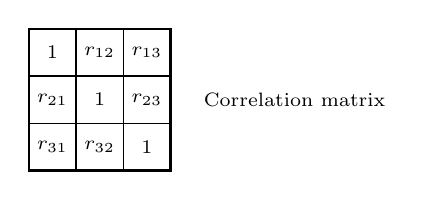
\begin{tikzpicture}[
  label/.style={font=\scriptsize},
]
% 3x3 correlation matrix sketch
\draw[thick] (0,0) rectangle (1.8,1.8);
\draw (0.6,0) -- (0.6,1.8);
\draw (1.2,0) -- (1.2,1.8);
\draw (0,0.6) -- (1.8,0.6);
\draw (0,1.2) -- (1.8,1.2);
\node[label] at (0.3,1.5) {1};
\node[label] at (0.9,1.5) {$r_{12}$};
\node[label] at (1.5,1.5) {$r_{13}$};
\node[label] at (0.3,0.9) {$r_{21}$};
\node[label] at (0.9,0.9) {1};
\node[label] at (1.5,0.9) {$r_{23}$};
\node[label] at (0.3,0.3) {$r_{31}$};
\node[label] at (0.9,0.3) {$r_{32}$};
\node[label] at (1.5,0.3) {1};
\node[label, right] at (2.1,0.9) {Correlation matrix};
\end{tikzpicture}
\end{visualbox}

\textbf{Key takeaways:} Know formulas + interpretations; correlation matrix is symmetric with 1s on the diagonal.
}

% 1.6 Basic Visualizations
\DefineTeach{1.6}{%
\begin{visualbox}
\centering
\includegraphics[width=0.9\linewidth]{asset/box-plot.png}
\end{visualbox}
}

% 1.7 Feature Transformations
\DefineTeach{1.7}{%
\begin{examlikelihood}{High}
Typical: pick the right transform (scale, log, encode) and explain why.
\end{examlikelihood}

\begin{examfavorite}
Identify data leakage in preprocessing; name the correct order for train/test transformations.
\end{examfavorite}

Why (motivation): Turn raw categorical/continuous variables into model-ready features.\\
What (definition): Encoding or discretizing features without changing the target meaning.\\
How (procedure/usage): Choose encoding by category type; choose binning by distribution.

\begin{cheatsheet}
\begin{itemize}
  \item \textbf{One-hot encoding:} create a 0/1 column per category (nominal).
  \item \textbf{Binary encoding:} represent categories as binary digits (compact one-hot).
  \item \textbf{Ordinal encoding:} map ordered categories to ranks (only if order is real).
  \item \textbf{Binning:} convert continuous to categories.
  \item \textbf{Equal-width binning:} fixed interval sizes across the range.
  \item \textbf{Equal-frequency binning:} same number of samples per bin.
\end{itemize}
\end{cheatsheet}

\begin{pitfall}
Fitting transforms on the full dataset (leakage). Always fit on training data, then apply to validation/test.
\end{pitfall}

\textbf{Key takeaways:} Use one-hot for nominal, ordinal for ordered labels, and binning for simplification.
}
